\documentclass[11pt,a4paper]{article}

% ---------- Paquetes ----------
\usepackage[utf8]{inputenc}
\usepackage[spanish,provide=*]{babel}
\usepackage[T1]{fontenc}
\usepackage[margin=2.5cm]{geometry}
\usepackage{graphicx}
\usepackage{booktabs}
\usepackage{longtable}
\usepackage{array}
\usepackage{xcolor}
\usepackage{enumitem}
\usepackage{hyperref}
\usepackage{fancyhdr}
\usepackage{titlesec}
\usepackage{amssymb}
\usepackage{placeins}
\usepackage{float}
\usepackage{tikz}
\usetikzlibrary{shapes.multipart,shapes.geometric,positioning,arrows.meta,calc,fit,backgrounds}

\hypersetup{
    colorlinks=true,
    urlcolor=black,
    linkcolor=black
}

\tikzset{
  umlclass/.style={rectangle split, rectangle split parts=3, draw=black, thick,
    rectangle split part align={left,left,left}, text width=4.6cm, font=\footnotesize, inner sep=4pt},
  assoc/.style={-, thick},
  mult/.style={font=\scriptsize},
  state/.style={rectangle, rounded corners=6pt, draw=black, thick, minimum width=2.6cm, minimum height=0.9cm, align=center, font=\small, fill=white},
  trans/.style={-{Stealth[length=2.2mm]}, thick},
  evt/.style={font=\scriptsize, align=center},
  initn/.style={circle, fill=black, minimum size=6pt, inner sep=0pt},
  finalst/.style={circle, draw=black, thick, minimum size=11pt, inner sep=0pt},
  finaldot/.style={circle, fill=black, minimum size=5.5pt, inner sep=0pt},
  act/.style={rectangle, rounded corners=6pt, draw=black, thick, minimum width=2.8cm, minimum height=0.9cm, align=center, font=\small}
}

\titleformat{\section}{\normalfont\Large\bfseries\color{black}}{P\thesection.}{0.5em}{}
\titlespacing*{\section}{0pt}{1.5em}{0.8em}

\setlength{\headheight}{14pt}
\pagestyle{fancy}
\fancyhf{}
\rhead{Prueba Práctica -- Unidad IV -- ISR-401}
\lhead{Sánchez Centeno Roselyn Andreina}
\rfoot{\thepage}

\newcolumntype{L}[1]{>{\raggedright\arraybackslash}p{#1}}

\title{\textbf{Prueba Práctica -- Unidad IV}\\[0.3em]
\large Validación, Gestión, Herramientas y Estándares de Requisitos\\[0.3em]
\normalsize Caso: Sistema de Gestión de Pedidos}
\author{Sánchez Centeno Roselyn Andreina \\ 4to Software ``A'' \\ Ingeniería de Requisitos (ISR-401) \\ Docente: Ing. Gleiston Guerrero, Mg.}
\date{Universidad Técnica Estatal de Quevedo \\ \today}

\begin{document}

\maketitle

\noindent\textbf{Repositorio del proyecto:} \url{https://github.com/Roselyn15/Ev_Practica_Unidad_IV_RS}

\vspace{1em}
\noindent\textbf{Caso práctico:} Una tienda en línea requiere un módulo para gestionar los pedidos
de sus clientes. Un \emph{Cliente} (cédula/RUC, nombre, correo) puede realizar cero o más \emph{Pedidos}.
Cada \emph{Pedido} (identificador, fecha, total) contiene una o más \emph{Líneas de pedido}, y cada línea
referencia un \emph{Producto} (código, descripción, precio, stock). Al registrar un pedido, el sistema
verifica la disponibilidad de stock: si hay existencias, confirma el pedido; si no, notifica el faltante.
Un pedido confirmado puede despacharse, luego entregarse, o bien anularse mientras no haya sido entregado.

\vspace{1em}
\hrule
\vspace{1em}

% ======================================================
\section{Modelo de datos -- Diagrama de clases UML}

Se identifican las clases \textbf{Cliente}, \textbf{Pedido}, \textbf{LineaPedido} y \textbf{Producto},
con sus atributos tipados, operaciones y multiplicidades en los extremos de las asociaciones
(\texttt{Cliente 1 -- * Pedido}, \texttt{Pedido 1 -- * LineaPedido}, \texttt{LineaPedido * -- 1 Producto}).

\begin{figure}[H]
    \centering
    \resizebox{0.95\textwidth}{!}{%
    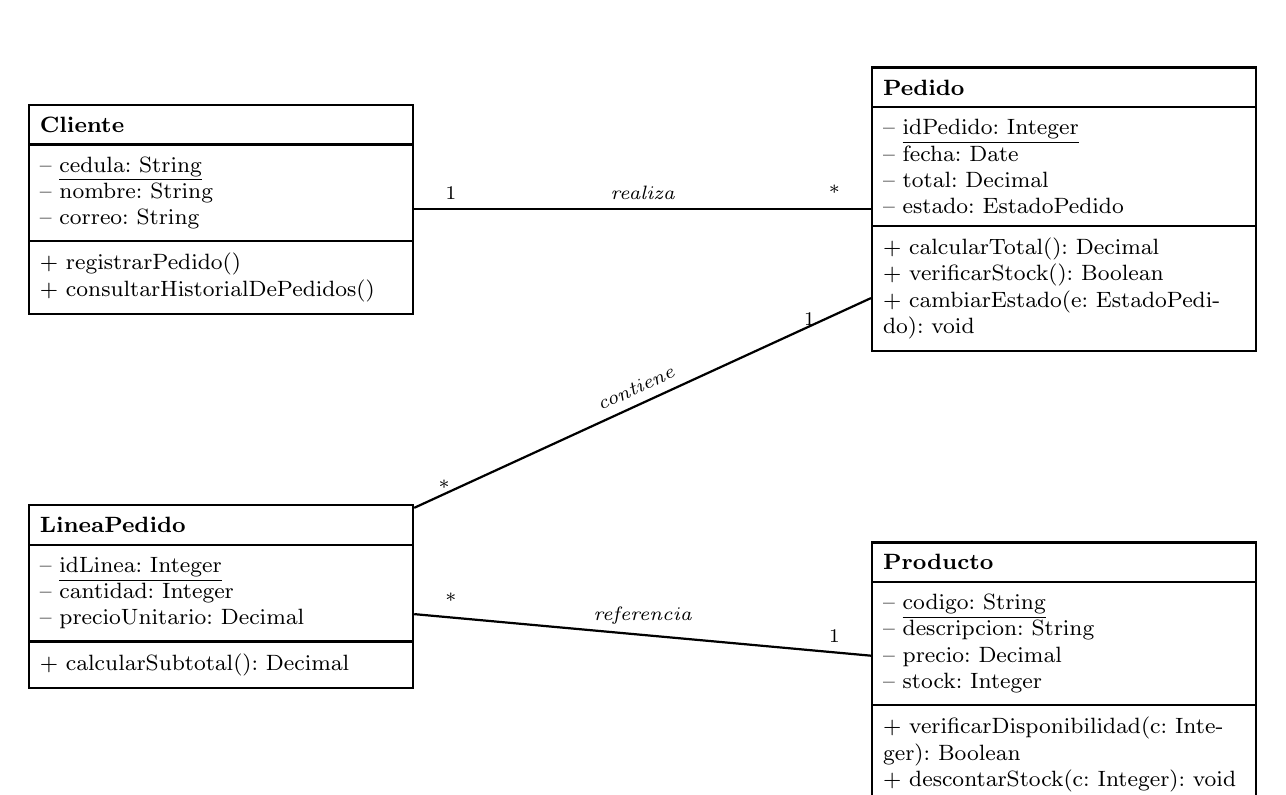
\begin{tikzpicture}[node distance=2.4cm and 3.6cm]

    \node[umlclass] (cliente) {
      \textbf{Cliente}
      \nodepart{two}
      -- \underline{cedula: String} \\
      -- nombre: String \\
      -- correo: String
      \nodepart{three}
      + registrarPedido() \\
      + consultarHistorialDePedidos()
    };

    \node[umlclass, right=of cliente, xshift=2.2cm] (pedido) {
      \textbf{Pedido}
      \nodepart{two}
      -- \underline{idPedido: Integer} \\
      -- fecha: Date \\
      -- total: Decimal \\
      -- estado: EstadoPedido
      \nodepart{three}
      + calcularTotal(): Decimal \\
      + verificarStock(): Boolean \\
      + cambiarEstado(e: EstadoPedido): void
    };

    \node[umlclass, below=of cliente] (linea) {
      \textbf{LineaPedido}
      \nodepart{two}
      -- \underline{idLinea: Integer} \\
      -- cantidad: Integer \\
      -- precioUnitario: Decimal
      \nodepart{three}
      + calcularSubtotal(): Decimal
    };

    \node[umlclass, below=of pedido] (producto) {
      \textbf{Producto}
      \nodepart{two}
      -- \underline{codigo: String} \\
      -- descripcion: String \\
      -- precio: Decimal \\
      -- stock: Integer
      \nodepart{three}
      + verificarDisponibilidad(c: Integer): Boolean \\
      + descontarStock(c: Integer): void
    };

    \draw[assoc] (cliente) -- (pedido)
      node[mult, pos=0.08, above] {1}
      node[mult, pos=0.92, above] {*}
      node[midway, above, font=\scriptsize\itshape] {realiza};

    \draw[assoc] (pedido) -- (linea)
      node[mult, pos=0.1, left] {1}
      node[mult, pos=0.9, left] {*}
      node[midway, sloped, above, font=\scriptsize\itshape] {contiene};

    \draw[assoc] (linea) -- (producto)
      node[mult, pos=0.08, above] {*}
      node[mult, pos=0.92, above] {1}
      node[midway, above, font=\scriptsize\itshape] {referencia};

    \end{tikzpicture}%
    }
    \caption{Diagrama de clases UML del dominio Sistema de Gestión de Pedidos (elaborado en TikZ, con asociaciones y multiplicidades explícitas).}
    \label{fig:p1}
\end{figure}

\FloatBarrier

% ======================================================
\section{Modelo funcional -- Diagrama de actividades UML}

Se modela el proceso \emph{Registrar pedido} usando dos carriles de responsabilidad: \textbf{Cliente}
y \textbf{Sistema}. Incluye nodo inicial, decisión sobre disponibilidad de stock, los dos caminos
alternativos (confirmar / notificar faltante), su convergencia y el nodo final.

\begin{figure}[H]
    \centering
    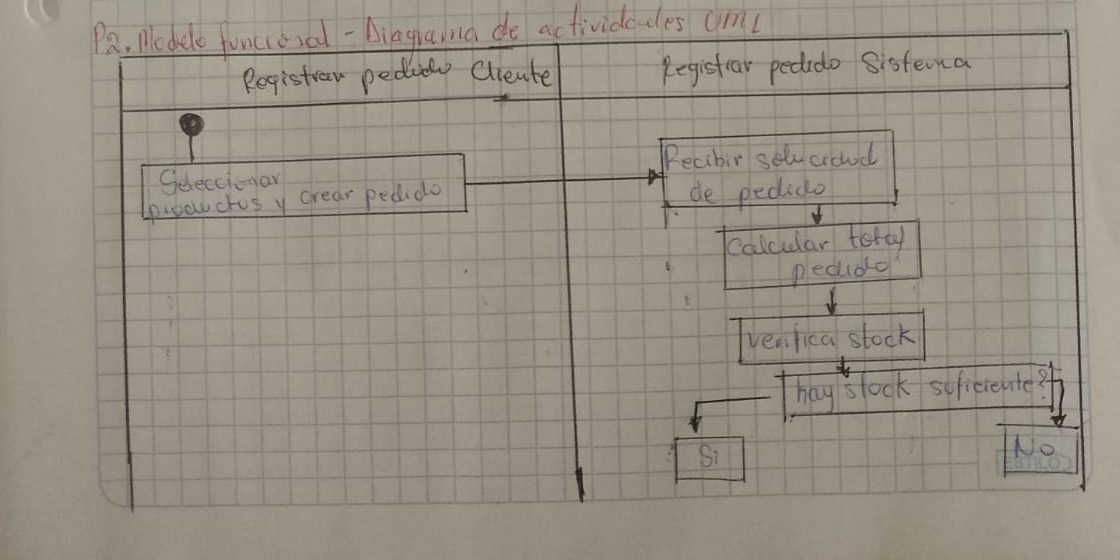
\includegraphics[width=0.95\textwidth]{figuras/p2_diagrama_actividades.png}
    \caption{Diagrama de actividades UML -- Registrar pedido (parte 1: solicitud, cálculo de total y verificación de stock).}
    \label{fig:p2a}
\end{figure}

\begin{figure}[H]
    \centering
    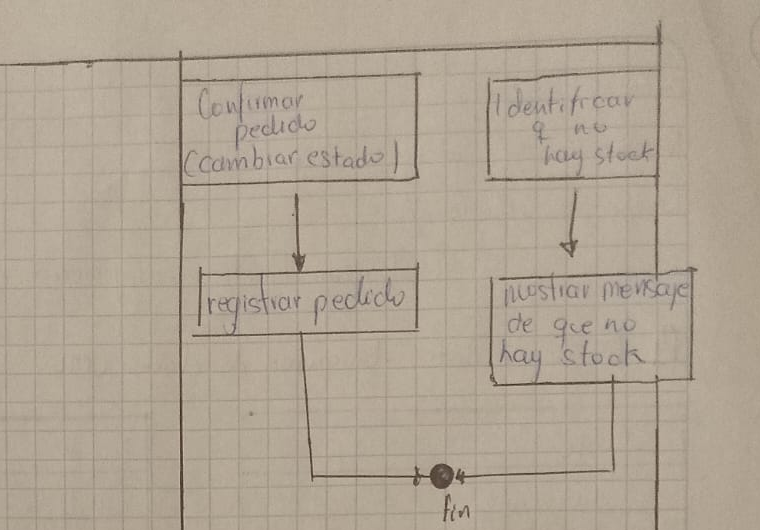
\includegraphics[width=0.8\textwidth]{figuras/p2b_diagrama_actividades_continuacion.png}
    \caption{Diagrama de actividades UML -- Registrar pedido (parte 2: continuación de los caminos ``Sí'' y ``No'' hasta el nodo final).}
    \label{fig:p2b}
\end{figure}

\FloatBarrier

% ======================================================
\section{Modelo de comportamiento -- Máquina de estados UML}

Ciclo de vida de un \textbf{Pedido}. Los estados \texttt{Confirmado} y \texttt{Enviado} se agrupan
en el superestado \texttt{EnProceso}, de modo que la transición \texttt{anular} se factoriza una
sola vez desde el borde del superestado hacia \texttt{Cancelado} (aplica mientras el pedido esté
confirmado o enviado, pero no una vez entregado). La transición \texttt{Registrado} $\to$
\texttt{Confirmado} lleva la guarda \texttt{[stock disponible]}; la transición
\texttt{Registrado} $\to$ \texttt{Cancelado} lleva la guarda \texttt{[stock no disponible]}.
\texttt{Entregado} y \texttt{Cancelado} son los dos estados finales de aceptación del proceso.

\begin{figure}[H]
    \centering
    \resizebox{0.98\textwidth}{!}{%
    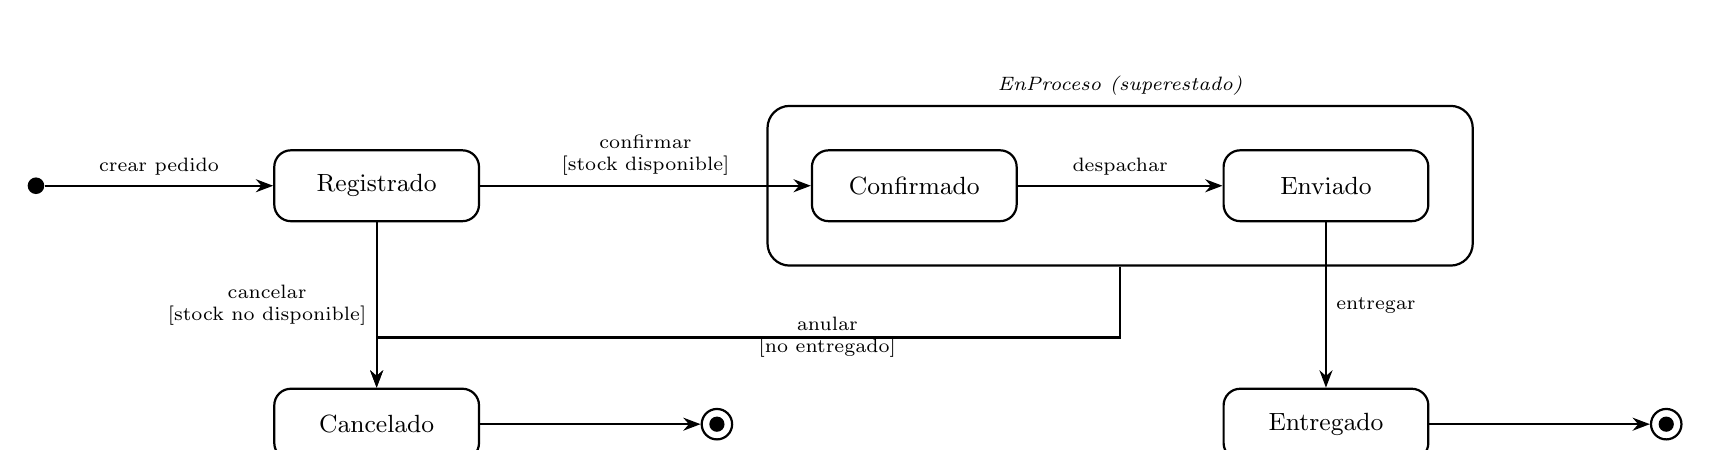
\begin{tikzpicture}[node distance=1.7cm and 2.6cm]

    \node[initn] (i0) {};
    \node[state, right=of i0, xshift=0.3cm] (reg) {Registrado};

    \node[state, right=of reg, xshift=1.6cm] (conf) {Confirmado};
    \node[state, right=of conf] (env) {Enviado};

    \begin{scope}[on background layer]
    \node[draw=black, thick, rounded corners=8pt, fit=(conf)(env), inner sep=0.55cm,
      label={[font=\scriptsize\itshape]above:EnProceso (superestado)}] (super) {};
    \end{scope}

    \node[state, below=of env, yshift=-0.4cm] (ent) {Entregado};
    \node[state, below=of reg, yshift=-0.4cm] (canc) {Cancelado};

    \node[finalst, right=of ent, xshift=0.2cm] (fEnt) {};
    \node[finaldot] at (fEnt) {};

    \node[finalst, right=of canc, xshift=0.2cm] (fCanc) {};
    \node[finaldot] at (fCanc) {};

    \draw[trans] (i0) -- (reg) node[evt, midway, above] {crear pedido};
    \draw[trans] (reg) -- (conf) node[evt, midway, above] {confirmar\\ {[stock disponible]}};
    \draw[trans] (reg) -- (canc) node[evt, midway, left] {cancelar\\ {[stock no disponible]}};
    \draw[trans] (conf) -- (env) node[evt, midway, above] {despachar};
    \draw[trans] (env) -- (ent) node[evt, midway, right] {entregar};
    \draw[trans] (super.south) -- ++(0,-0.9) -| (canc.north)
      node[evt, pos=0.25, right] {anular\\ {[no entregado]}};
    \draw[trans] (ent) -- (fEnt);
    \draw[trans] (canc) -- (fCanc);

    \end{tikzpicture}%
    }
    \caption{Máquina de estados UML del ciclo de vida de un Pedido, con superestado \texttt{EnProceso}, guardas y estados finales.}
    \label{fig:p3}
\end{figure}

\FloatBarrier

% ======================================================
\section{Consistencia entre las tres perspectivas}

\begin{table}[H]
\centering
\begin{tabular}{L{3cm} L{5.5cm} L{4.5cm}}
\toprule
\textbf{Evento (P3)} & \textbf{Función/acción (P2)} & \textbf{Entidad/atributo (P1)} \\
\midrule
registrar  & Recibir solicitud de pedido               & \texttt{Pedido} (creación) \\
despachar  & \emph{sin función explícita en P2}        & \texttt{Pedido.estado = Enviado} \\
confirmar  & Confirmar pedido (cambiar estado)         & \texttt{Pedido.estado = Confirmado} \\
cancelar   & Identificar que no hay stock              & \texttt{Pedido.estado = Cancelado} \\
entregar   & \emph{sin función explícita en P2}         & \texttt{Pedido.estado = Entregado} \\
\bottomrule
\end{tabular}
\caption{Tabla de verificación cruzada entre eventos, funciones y entidades.}
\end{table}

\textbf{Defecto detectado:} los eventos \texttt{despachar} y \texttt{entregar} de la máquina de
estados (P3) no tienen una función/acción correspondiente en el diagrama de actividades (P2), el
cual solo modela el subproceso de \emph{registro} del pedido. Esto constituye una inconsistencia
entre los modelos, ya que P3 define transiciones para las cuales P2 no describe el comportamiento.

\textbf{Corrección aplicada:} se extiende el modelo funcional (P2) agregando las actividades
faltantes \emph{Despachar pedido} y \emph{Entregar pedido} en el carril del Sistema, de modo que
todos los eventos de la máquina de estados (P3) queden representados en el diagrama de actividades.

\begin{figure}[H]
    \centering
    \resizebox{0.98\textwidth}{!}{%
    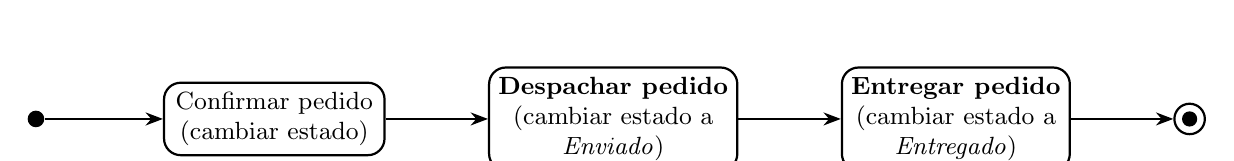
\begin{tikzpicture}[node distance=1.4cm and 1.3cm]
    \node[initn] (i) {};
    \node[act, right=of i, xshift=0.2cm] (a1) {Confirmar pedido\\ (cambiar estado)};
    \node[act, right=of a1] (a2) {\textbf{Despachar pedido}\\ (cambiar estado a\\ \emph{Enviado})};
    \node[act, right=of a2] (a3) {\textbf{Entregar pedido}\\ (cambiar estado a\\ \emph{Entregado})};
    \node[finalst, right=of a3] (f) {};
    \node[finaldot] at (f) {};

    \draw[trans] (i) -- (a1);
    \draw[trans] (a1) -- (a2);
    \draw[trans] (a2) -- (a3);
    \draw[trans] (a3) -- (f);
    \end{tikzpicture}%
    }
    \caption{Fragmento corregido del diagrama de actividades (P2): actividades ``Despachar pedido'' y ``Entregar pedido'' añadidas en el carril del Sistema, cerrando la inconsistencia detectada.}
    \label{fig:p4-correccion}
\end{figure}

\FloatBarrier

% ======================================================
\section{Especificación de requisitos con esquema de atributos}

\subsection*{Requisitos funcionales}
\begin{enumerate}[label=\textbf{RF-\arabic*}]
    \item Los pedidos deben ser registrados en el sistema por el cliente, dado que existe stock suficiente de los productos solicitados.
    \item Los datos personales del cliente (cédula, nombre, correo) registrados en un pedido deben mantenerse protegidos frente a accesos no autorizados.
\end{enumerate}

\subsection*{Requisitos no funcionales}
\begin{enumerate}[label=\textbf{RNF-\arabic*}]
    \item \emph{Eficiencia de desempeño (ISO/IEC 25010:2023):} el sistema debe registrar un pedido en un tiempo de respuesta menor a 0.2 segundos.
    \item \emph{Seguridad (ISO/IEC 25010:2023):} el sistema debe cifrar los datos personales del cliente almacenados, garantizando su confidencialidad.
\end{enumerate}

\begin{table}[H]
\centering
\small
\begin{tabular}{L{1.6cm} L{2cm} L{1.8cm} L{1.6cm} L{2cm} L{1.3cm} L{3.2cm}}
\toprule
\textbf{ID} & \textbf{Prioridad} & \textbf{Estado} & \textbf{Fuente} & \textbf{Estabilidad} & \textbf{Versión} & \textbf{Verificación} \\
\midrule
RF-1  & Alta & Propuesto & Caso de negocio & Estable & 1.0 & Prueba funcional de registro \\
RF-2  & Alta & Propuesto & Regulación de datos & Estable & 1.0 & Inspección de control de acceso \\
RNF-1 & Media & Propuesto & Cliente & Estable & 1.0 & Prueba de rendimiento (cronometraje) \\
RNF-2 & Alta & Propuesto & Normativa de seguridad & Estable & 1.0 & Auditoría de cifrado \\
\bottomrule
\end{tabular}
\caption{Esquema de atributos de los requisitos.}
\end{table}

\FloatBarrier

% ======================================================
\section{Priorización MoSCoW}

\begin{table}[H]
\centering
\begin{tabular}{l c c c c L{5cm}}
\toprule
\textbf{R\#} & \textbf{Must} & \textbf{Should} & \textbf{Could} & \textbf{Won't have} & \textbf{Justificación} \\
\midrule
RF-1  & \checkmark & & & & Sin registro de pedidos no existe el producto mínimo viable. \\
RF-2  & \checkmark & & & & Proteger datos personales es obligación legal y de confianza del cliente. \\
RNF-1 & & \checkmark & & & Mejora la experiencia, pero el sistema es viable con una latencia algo mayor. \\
RNF-2 & & & \checkmark & & Deseable reforzar el cifrado; puede incorporarse en una iteración posterior sin bloquear el lanzamiento. \\
\bottomrule
\end{tabular}
\caption{Clasificación MoSCoW de los requisitos (RF-1 y RF-2 son Must have).}
\end{table}

\FloatBarrier

% ======================================================
\section{Validación por inspección (checklist ISO/IEC/IEEE 29148)}

\subsection*{Paso 1: identificación de defectos (sin corregir)}
\begin{table}[H]
\centering
\begin{tabular}{l l L{9cm}}
\toprule
\textbf{Requisito} & \textbf{Propiedad evaluada} & \textbf{Defecto detectado} \\
\midrule
RF-1  & Completo   & El tiempo/condición de disponibilidad de stock no queda del todo exacto ni cuantificado. \\
RF-2  & Singular   & No se especifica \emph{cómo} deben estar protegidos los datos (mecanismo no definido). \\
RNF-1 & Factible   & Es claro lo que se pide, pero la meta de 0.2s puede ser difícil de sustentar sin más contexto técnico. \\
RNF-2 & Verificable & Se asume que el cifrado ya estaría integrado en el sistema, sin un criterio de verificación explícito. \\
\bottomrule
\end{tabular}
\caption{Defectos detectados por inspección (identificación separada de la corrección).}
\end{table}

\subsection*{Paso 2: retrabajo (requisitos corregidos)}
\begin{enumerate}[label=\textbf{RF-\arabic*'}]
    \item El sistema debe registrar un pedido únicamente cuando exista stock suficiente para todos los productos solicitados, verificando la disponibilidad antes de confirmar.
    \item Los datos personales del cliente deben almacenarse cifrados en reposo (AES-256) y transmitirse mediante un canal seguro (TLS 1.2 o superior).
\end{enumerate}
\begin{enumerate}[label=\textbf{RNF-\arabic*'}]
    \item El sistema debe registrar un pedido en un tiempo de respuesta menor o igual a 0.2 segundos, medido bajo condiciones de carga normal (percentil 95).
    \item El sistema debe cifrar los datos personales del cliente y este control debe verificarse mediante auditoría de seguridad semestral.
\end{enumerate}

\FloatBarrier

% ======================================================
\section{Pruebas de aceptación trazadas}

\begin{table}[H]
\centering
\small
\begin{tabular}{l l L{3.2cm} L{3.2cm} l}
\toprule
\textbf{Prueba} & \textbf{Tipo} & \textbf{Entradas} & \textbf{Criterio de éxito} & \textbf{Traza a} \\
\midrule
PA-01 & Funcional      & Pedido con productos en stock              & El pedido queda registrado y confirmado & RF-1 \\
PA-02 & Funcional      & Solicitud de acceso a datos de un cliente  & El acceso es denegado sin autorización  & RF-2 \\
PA-03 & No funcional   & Registro de 100 pedidos concurrentes       & Tiempo de respuesta $\leq$ 0.2s en el 95\% de los casos & RNF-1 \\
PA-04 & No funcional / Regresión & Inspección de la base de datos tras un despliegue & Los campos personales se almacenan cifrados & RNF-2 \\
\bottomrule
\end{tabular}
\caption{Pruebas de aceptación trazadas a cada requisito de P5.}
\end{table}

\FloatBarrier

\end{document}
